\documentclass[letterpaper,journal]{ieeetran}

\usepackage[utf8]{inputenc}
\usepackage[spanish]{babel}
\usepackage{fullpage}
\usepackage{graphicx}
\usepackage{caption}
\usepackage{subcaption}
\usepackage{amsmath}
\usepackage{float}
\usepackage{pgf}
\usepackage{tikz}
\usepackage{xcolor}
\usepackage{color}
\usepackage{amssymb}
\usepackage{caption}
\usepackage{subcaption}

%\usepackage{lmodern}
%\renewcommand*\familydefault{\sfdefault} %% Only if the base font of the document is to be sans serif
%\usepackage[T1]{fontenc}


\title{Conceptos de Automatización}
\author{Antonio D. Vásquez Briones\\ \texttt{antonio.vasquez03}@\texttt{inacapmail.cl}}
\date{\today}


\begin{document}
\maketitle
\section{Automatización}
En general, cuando se habla de \emph{Automatización} inmediatamente se asocia el concepto a sistemas inteligentes, sistemas que realizan tareas repetida e incansablemente o sistemas que controlan alguna variable de interés, como por ejemplo puertas de recintos comerciales que se abren cuando algún cliente se acerca a ellas, rápidas lineas de ensamblaje que completan varias tareas al minuto o un climatizador que mantiene la temperatura que el usuario quiera independiente de las condiciones ambientales exteriores; son todos sistemas automáticos que en cierta medida no requieren la intervención de un ser humano para su pleno funcionamiento.
\vspace{10pt}

\textbf{Automático}
\begin{quotation}
	\it
	Que funciona por sí solo o que realiza total o parcialmente un proceso sin ayuda humana.
\end{quotation}
\vspace{10pt}
Es posible diferenciar dos tipos de sistemas que tienen propósitos diferentes pero no dejan de ser automáticos. Por ejemplo 
\begin{itemize}
	\item Se tiene un estanque con dos botones que al ser presionados comanda el vaciado o llenado completo del recipiente.
	\begin{center}
		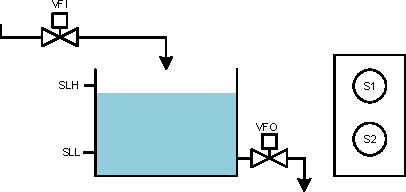
\includegraphics[scale=0.8]{Estanque.pdf}
	\end{center}
	
	\item Se tiene un sistema que controla el nivel del estanque que es capaz de purgar los excesos de nivel perdido mediante la apertura gradual de una válvula.
	\begin{center}
		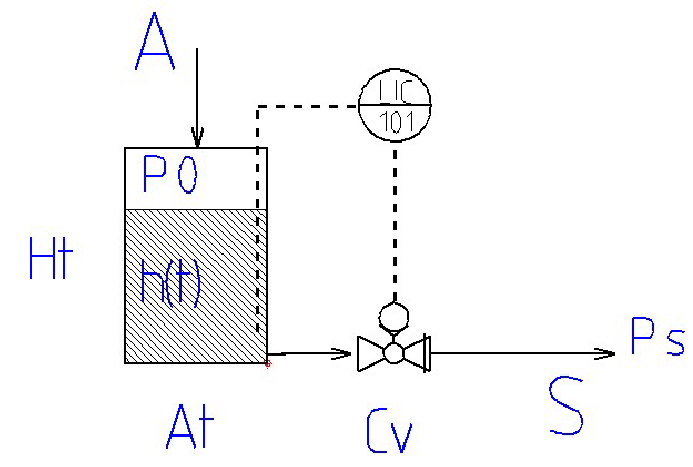
\includegraphics[scale=0.23]{EstanqueControl.png}
	\end{center}
	
	La diferencia fundamental entre estos dos sistemas, es que uno automatiza una \emph{tarea} mientras que el otro realiza una \emph{regulación} automática permanente en el tiempo.
	
	\section{Control de Eventos Discretos}
	Es la automatización de tareas repetitivas y eventos discretos que no requieren mayor inteligencia, por lo que pueden ser ejecutados por maquinas de forma reiterativa y a gran velocidad. Se dividen en tareas y eventos que tienen un comienzo y un final. Dentro de este tipo de sistemas se encuentran.
	\begin{itemize}
		\item Partidas directas e inversores de giro con elementos de comando eléctrico.
		\item Encender o apagar las luces de una vivienda a horarios determinados.
		\item Encender o apagar las luminarias en la vía pública cuando se ha escondido el sol.
		\item Ensamblar piezas mediante brazos robóticos.
	\end{itemize}	
	
	\section{Control Regulatorio}
	
	Consiste en mantener variables físicas en un valor deseado según estrategias acuñadas por la \emph{Teoría de Control} que generalmente requieren un análisis matemático avanzado de la física que involucra el proceso que se quiere controlar.
	
	En su forma más básica, el control regulatorio se logra siguiendo la \emph{Estructura General de Control} detallada a continuación.
	
	\section[Control Regulatorio]{Estructura general de control.}
	Al representar las distintas partes del sistema como bloques las partes necesarias para controlar una variable junto con las interconexiones entre las mismas son las siguientes. 
	
	\begin{center}
		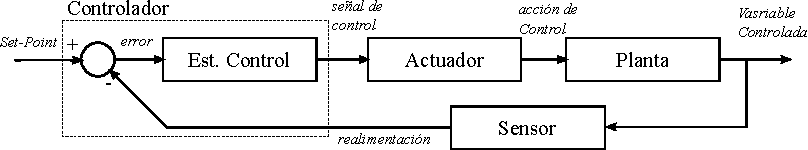
\includegraphics[scale=0.6]{egControl.pdf}
	\end{center}
	\subsection{Bloques del Sistema}
	
	\subsubsection{Controlador}
	Es un equipo al que se ingresa el valor de set point, se conecta el sensor y el actuador. Contiene la Estrategía de Control y en base a esta comanda al actuador según la magnitud de la diferencia entre el valor deseado y el valor actual que mide el sensor.
	
	\subsubsection{Actuador}
	Es el encargado de ejercer la  \emph{Acción de Control}, es comandado por el controlador y es el que provee el esfuerzo necesario para cambiar el estado actual de la variable de salida del proceso. Se conoce tambien con el nombre de \emph{Elemento Final de Control}.
	
	\subsubsection{Proceso}
	Comunmente se le llama \emph{Planta}, y es el proceso físico que se quiere controlar, por ejemlo un estanque con su dinámica de llenado y vaciado, una caldera con toda la física involucrada en el calentamiento del agua y su transformación a vapor. Este bloque, recibe la acción de control cambiando su estado, siendo este medido por el sensor e informando al controlador.
	
	\subsubsection{Sensor}
	Se encarga de informar al controlador acerca del estado actual del proceso que se quiere controlar, es el encargado de producir la \emph{Realimentación} necesaria para que el sistema sea controlado.
	
	\subsection{Señales del Sistema}
	
	Son las líneas que interconectan cada uno de los bloques.
	
	\subsubsection{Set-Point} Es el valor deseado para el sistema en cuestión, tiene la misma magnitud que la variable de salida, por ejemplo si se controla el nivel de un estanque, el set point, será un nivel determinado, por ejemplo 5m de altura. También se conoce con los nombres de \emph{Señal de Consigna}, \emph{Señal de Referencia}, \emph{Entrada del Sistema}, entre otros.
	
	\subsubsection{Error} Es el valor resultante de la resta del Set-point con el Valor actual del proceso informado por realimentación que provee el sensor. Cuando este valor es cero se dice que el sistema esta controlado.
	
	\subsubsection{Señal de Control} Es la señal de comando para el actuador  generada en el controlador de acuerdo al error calculado según lo que dicte la estrategia de control.
	
	\subsubsection{Acción de control} Es el esfuerzo físico que ejerce el actuador, puede ser cerrar una válvula, encender un calefactor, encender un ventilador, etc.
	
	\subsubsection{Realimentación} Es la señal electrica enviada por el sensor para informar al controlador el estado actual de la planta.
\end{itemize}
\end{document}